% Requires \usepackage{graphicx}; adjust the PDF path if needed.
% Native size: 180 x 84 mm. The figure* environment spans both columns.
\begin{figure*}[t]
  \centering
  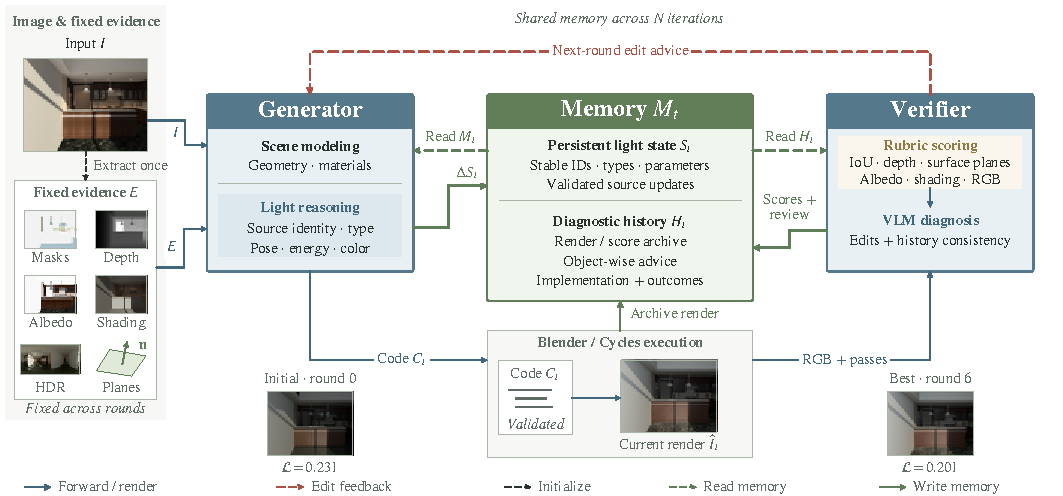
\includegraphics[width=\textwidth]{lightproxy_method_v3.pdf}
  \caption{Overview of the generator--memory--verifier reconstruction loop.
  The generator uses the reference image, fixed visual evidence, and shared
  memory to model scene geometry and materials and reason about light sources.
  Central memory separates persistent light state $S_t$ from diagnostic history
  $H_t$: the generator reads both and submits validated state changes, while
  the verifier reads historical context and records scores and diagnoses.
  Blender/Cycles executes the generated code and produces an RGB image and
  diagnostic passes. The verifier combines deterministic rubric scoring with
  VLM diagnosis, yielding edit advice for the next iteration. Rendered
  observations are archived for later comparison. The process runs for a
  fixed budget of $N$ iterations and exports the completed round with the
  lowest fixed-weight selection loss. The small initial and best-round
  images show actual outputs from one archived run; lower $\mathcal{L}$ is
  better.}
  \label{fig:method}
\end{figure*}
